% Options for packages loaded elsewhere
\PassOptionsToPackage{unicode}{hyperref}
\PassOptionsToPackage{hyphens}{url}
\documentclass[
  11pt,
]{article}
\usepackage{xcolor}
\usepackage[margin=1in]{geometry}
\usepackage{amsmath,amssymb}
\setcounter{secnumdepth}{5}
\usepackage{iftex}
\ifPDFTeX
  \usepackage[T1]{fontenc}
  \usepackage[utf8]{inputenc}
  \usepackage{textcomp} % provide euro and other symbols
\else % if luatex or xetex
  \usepackage{unicode-math} % this also loads fontspec
  \defaultfontfeatures{Scale=MatchLowercase}
  \defaultfontfeatures[\rmfamily]{Ligatures=TeX,Scale=1}
\fi
\usepackage{lmodern}
\ifPDFTeX\else
  % xetex/luatex font selection
\fi
% Use upquote if available, for straight quotes in verbatim environments
\IfFileExists{upquote.sty}{\usepackage{upquote}}{}
\IfFileExists{microtype.sty}{% use microtype if available
  \usepackage[]{microtype}
  \UseMicrotypeSet[protrusion]{basicmath} % disable protrusion for tt fonts
}{}
\makeatletter
\@ifundefined{KOMAClassName}{% if non-KOMA class
  \IfFileExists{parskip.sty}{%
    \usepackage{parskip}
  }{% else
    \setlength{\parindent}{0pt}
    \setlength{\parskip}{6pt plus 2pt minus 1pt}}
}{% if KOMA class
  \KOMAoptions{parskip=half}}
\makeatother
\usepackage{color}
\usepackage{fancyvrb}
\newcommand{\VerbBar}{|}
\newcommand{\VERB}{\Verb[commandchars=\\\{\}]}
\DefineVerbatimEnvironment{Highlighting}{Verbatim}{commandchars=\\\{\}}
% Add ',fontsize=\small' for more characters per line
\usepackage{framed}
\definecolor{shadecolor}{RGB}{248,248,248}
\newenvironment{Shaded}{\begin{snugshade}}{\end{snugshade}}
\newcommand{\AlertTok}[1]{\textcolor[rgb]{0.94,0.16,0.16}{#1}}
\newcommand{\AnnotationTok}[1]{\textcolor[rgb]{0.56,0.35,0.01}{\textbf{\textit{#1}}}}
\newcommand{\AttributeTok}[1]{\textcolor[rgb]{0.13,0.29,0.53}{#1}}
\newcommand{\BaseNTok}[1]{\textcolor[rgb]{0.00,0.00,0.81}{#1}}
\newcommand{\BuiltInTok}[1]{#1}
\newcommand{\CharTok}[1]{\textcolor[rgb]{0.31,0.60,0.02}{#1}}
\newcommand{\CommentTok}[1]{\textcolor[rgb]{0.56,0.35,0.01}{\textit{#1}}}
\newcommand{\CommentVarTok}[1]{\textcolor[rgb]{0.56,0.35,0.01}{\textbf{\textit{#1}}}}
\newcommand{\ConstantTok}[1]{\textcolor[rgb]{0.56,0.35,0.01}{#1}}
\newcommand{\ControlFlowTok}[1]{\textcolor[rgb]{0.13,0.29,0.53}{\textbf{#1}}}
\newcommand{\DataTypeTok}[1]{\textcolor[rgb]{0.13,0.29,0.53}{#1}}
\newcommand{\DecValTok}[1]{\textcolor[rgb]{0.00,0.00,0.81}{#1}}
\newcommand{\DocumentationTok}[1]{\textcolor[rgb]{0.56,0.35,0.01}{\textbf{\textit{#1}}}}
\newcommand{\ErrorTok}[1]{\textcolor[rgb]{0.64,0.00,0.00}{\textbf{#1}}}
\newcommand{\ExtensionTok}[1]{#1}
\newcommand{\FloatTok}[1]{\textcolor[rgb]{0.00,0.00,0.81}{#1}}
\newcommand{\FunctionTok}[1]{\textcolor[rgb]{0.13,0.29,0.53}{\textbf{#1}}}
\newcommand{\ImportTok}[1]{#1}
\newcommand{\InformationTok}[1]{\textcolor[rgb]{0.56,0.35,0.01}{\textbf{\textit{#1}}}}
\newcommand{\KeywordTok}[1]{\textcolor[rgb]{0.13,0.29,0.53}{\textbf{#1}}}
\newcommand{\NormalTok}[1]{#1}
\newcommand{\OperatorTok}[1]{\textcolor[rgb]{0.81,0.36,0.00}{\textbf{#1}}}
\newcommand{\OtherTok}[1]{\textcolor[rgb]{0.56,0.35,0.01}{#1}}
\newcommand{\PreprocessorTok}[1]{\textcolor[rgb]{0.56,0.35,0.01}{\textit{#1}}}
\newcommand{\RegionMarkerTok}[1]{#1}
\newcommand{\SpecialCharTok}[1]{\textcolor[rgb]{0.81,0.36,0.00}{\textbf{#1}}}
\newcommand{\SpecialStringTok}[1]{\textcolor[rgb]{0.31,0.60,0.02}{#1}}
\newcommand{\StringTok}[1]{\textcolor[rgb]{0.31,0.60,0.02}{#1}}
\newcommand{\VariableTok}[1]{\textcolor[rgb]{0.00,0.00,0.00}{#1}}
\newcommand{\VerbatimStringTok}[1]{\textcolor[rgb]{0.31,0.60,0.02}{#1}}
\newcommand{\WarningTok}[1]{\textcolor[rgb]{0.56,0.35,0.01}{\textbf{\textit{#1}}}}
\usepackage{graphicx}
\makeatletter
\newsavebox\pandoc@box
\newcommand*\pandocbounded[1]{% scales image to fit in text height/width
  \sbox\pandoc@box{#1}%
  \Gscale@div\@tempa{\textheight}{\dimexpr\ht\pandoc@box+\dp\pandoc@box\relax}%
  \Gscale@div\@tempb{\linewidth}{\wd\pandoc@box}%
  \ifdim\@tempb\p@<\@tempa\p@\let\@tempa\@tempb\fi% select the smaller of both
  \ifdim\@tempa\p@<\p@\scalebox{\@tempa}{\usebox\pandoc@box}%
  \else\usebox{\pandoc@box}%
  \fi%
}
% Set default figure placement to htbp
\def\fps@figure{htbp}
\makeatother
\setlength{\emergencystretch}{3em} % prevent overfull lines
\providecommand{\tightlist}{%
  \setlength{\itemsep}{0pt}\setlength{\parskip}{0pt}}
\usepackage{amsmath}
% Shared LaTeX preamble for all Data Mining / ISLR chapter documents.
% Provides \makecoverpage{<assignment title>} — a standalone title page
% with fixed student identity, so every chapter/lab looks uniform.

\usepackage{graphicx}

\newcommand{\makecoverpage}[1]{%
\begin{titlepage}
\centering
\vspace*{2cm}

{\Large \textbf{Adventist University of Central Africa}}\\[0.4cm]
{\large Master's in Big Data Analytics}\\[2cm]

{\Huge \textbf{#1}}\\[0.5cm]
{\large \textit{Introduction to Statistical Learning with Applications in R}}\\[3cm]

\begin{tabular}{rl}
\textbf{Programme:} & MSc Big Data Analytics \\
\textbf{Course Title:} & Data Mining \\
\textbf{Course Code:} & MSDA 9124 \\
\textbf{Lecturer:} & Dr. Pacifique Nizeyimana \\
\textbf{Student Name:} & Wayne Rubangisa \\
\textbf{Student ID:} & 101220 \\
\end{tabular}

\vfill

{\large September 2026}

\end{titlepage}
}

\usepackage{bookmark}
\IfFileExists{xurl.sty}{\usepackage{xurl}}{} % add URL line breaks if available
\urlstyle{same}
\hypersetup{
  hidelinks,
  pdfcreator={LaTeX via pandoc}}

\author{}
\date{\vspace{-2.5em}}

\begin{document}

\makecoverpage{Chapter 3 --- Linear Regression \\ Lab}

\section{Introduction}\label{introduction}

This lab walks through fitting and interpreting linear regression models
in R, following the workflow used in Chapter 3 of \emph{An Introduction
to Statistical Learning}. We'll cover:

\begin{itemize}
\tightlist
\item
  Simple linear regression
\item
  Confidence and prediction intervals
\item
  Diagnostic plots for checking model assumptions
\item
  Multiple linear regression
\item
  Interaction terms
\item
  Non-linear transformations of predictors
\item
  Qualitative (categorical) predictors
\item
  Writing a small reusable function
\end{itemize}

We'll use two classic datasets that ship with the \texttt{ISLR2}
package: \texttt{Boston} (housing values in the suburbs of Boston) and
\texttt{Carseats} (simulated child car seat sales data).

\subsection{Required packages}\label{required-packages}

\begin{Shaded}
\begin{Highlighting}[]
\CommentTok{\# install.packages(c("MASS", "ISLR2", "car"))  \# uncomment if needed}
\FunctionTok{library}\NormalTok{(MASS)     }\CommentTok{\# for some classic datasets and stats utilities}
\FunctionTok{library}\NormalTok{(ISLR2)    }\CommentTok{\# Boston and Carseats datasets live here (2nd edition)}
\FunctionTok{library}\NormalTok{(car)      }\CommentTok{\# for vif() {-}{-} variance inflation factors}
\end{Highlighting}
\end{Shaded}

\begin{quote}
\textbf{Note:} In the 2nd edition of ISLR, the \texttt{Boston} dataset
moved from the \texttt{MASS} package into \texttt{ISLR2}. Loading both
packages avoids ambiguity issues; if you have both loaded,
\texttt{ISLR2::Boston} is the one used below.
\end{quote}

\section{Simple Linear Regression}\label{simple-linear-regression}

We start by exploring the relationship between \texttt{medv} (median
home value, in \$1000s) and \texttt{lstat} (percentage of the population
with ``lower status'', e.g. lower income/education) in the
\texttt{Boston} data set.

\begin{Shaded}
\begin{Highlighting}[]
\NormalTok{Boston }\OtherTok{\textless{}{-}}\NormalTok{ ISLR2}\SpecialCharTok{::}\NormalTok{Boston}
\FunctionTok{str}\NormalTok{(Boston)}
\end{Highlighting}
\end{Shaded}

\begin{verbatim}
## 'data.frame':    506 obs. of  13 variables:
##  $ crim   : num  0.00632 0.02731 0.02729 0.03237 0.06905 ...
##  $ zn     : num  18 0 0 0 0 0 12.5 12.5 12.5 12.5 ...
##  $ indus  : num  2.31 7.07 7.07 2.18 2.18 2.18 7.87 7.87 7.87 7.87 ...
##  $ chas   : int  0 0 0 0 0 0 0 0 0 0 ...
##  $ nox    : num  0.538 0.469 0.469 0.458 0.458 0.458 0.524 0.524 0.524 0.524 ...
##  $ rm     : num  6.58 6.42 7.18 7 7.15 ...
##  $ age    : num  65.2 78.9 61.1 45.8 54.2 58.7 66.6 96.1 100 85.9 ...
##  $ dis    : num  4.09 4.97 4.97 6.06 6.06 ...
##  $ rad    : int  1 2 2 3 3 3 5 5 5 5 ...
##  $ tax    : num  296 242 242 222 222 222 311 311 311 311 ...
##  $ ptratio: num  15.3 17.8 17.8 18.7 18.7 18.7 15.2 15.2 15.2 15.2 ...
##  $ lstat  : num  4.98 9.14 4.03 2.94 5.33 ...
##  $ medv   : num  24 21.6 34.7 33.4 36.2 28.7 22.9 27.1 16.5 18.9 ...
\end{verbatim}

\begin{Shaded}
\begin{Highlighting}[]
\FunctionTok{names}\NormalTok{(Boston)}
\end{Highlighting}
\end{Shaded}

\begin{verbatim}
##  [1] "crim"    "zn"      "indus"   "chas"    "nox"     "rm"      "age"    
##  [8] "dis"     "rad"     "tax"     "ptratio" "lstat"   "medv"
\end{verbatim}

\subsection{Fitting the model}\label{fitting-the-model}

Before fitting anything, it's worth being explicit about what
\texttt{lm()} is actually estimating. A simple linear regression assumes
the true relationship has the form

\[
\text{medv} = \beta_0 + \beta_1 \cdot \text{lstat} + \epsilon
\]

where \(\beta_0\) and \(\beta_1\) are unknown population parameters and
\(\epsilon\) is irreducible error. \texttt{lm()} doesn't know
\(\beta_0\) and \(\beta_1\) --- it estimates them, \(\hat\beta_0\) and
\(\hat\beta_1\), by finding the line that minimizes the residual sum of
squares over the \(n\) observed pairs \((x_i, y_i)\):

\[
\text{RSS} = \sum_{i=1}^{n} \left(y_i - \hat\beta_0 - \hat\beta_1 x_i\right)^2
\]

which has the closed-form (least-squares) solution

\[
\hat\beta_1 = \frac{\sum_{i=1}^n (x_i - \bar{x})(y_i - \bar{y})}{\sum_{i=1}^n (x_i - \bar{x})^2}, \qquad
\hat\beta_0 = \bar{y} - \hat\beta_1 \bar{x}
\]

\begin{Shaded}
\begin{Highlighting}[]
\NormalTok{lm.fit }\OtherTok{\textless{}{-}} \FunctionTok{lm}\NormalTok{(medv }\SpecialCharTok{\textasciitilde{}}\NormalTok{ lstat, }\AttributeTok{data =}\NormalTok{ Boston)}
\NormalTok{lm.fit}
\end{Highlighting}
\end{Shaded}

\begin{verbatim}
## 
## Call:
## lm(formula = medv ~ lstat, data = Boston)
## 
## Coefficients:
## (Intercept)        lstat  
##       34.55        -0.95
\end{verbatim}

\begin{Shaded}
\begin{Highlighting}[]
\FunctionTok{summary}\NormalTok{(lm.fit)}
\end{Highlighting}
\end{Shaded}

\begin{verbatim}
## 
## Call:
## lm(formula = medv ~ lstat, data = Boston)
## 
## Residuals:
##     Min      1Q  Median      3Q     Max 
## -15.168  -3.990  -1.318   2.034  24.500 
## 
## Coefficients:
##             Estimate Std. Error t value Pr(>|t|)    
## (Intercept) 34.55384    0.56263   61.41   <2e-16 ***
## lstat       -0.95005    0.03873  -24.53   <2e-16 ***
## ---
## Signif. codes:  0 '***' 0.001 '**' 0.01 '*' 0.05 '.' 0.1 ' ' 1
## 
## Residual standard error: 6.216 on 504 degrees of freedom
## Multiple R-squared:  0.5441, Adjusted R-squared:  0.5432 
## F-statistic: 601.6 on 1 and 504 DF,  p-value: < 2.2e-16
\end{verbatim}

The output above gives us \(\hat\beta_0\) and \(\hat\beta_1\) (under
\texttt{Estimate}), their standard errors, t-statistics, and p-values,
along with two summary measures of overall fit:

\[
R^2 = 1 - \frac{\text{RSS}}{\text{TSS}}, \qquad
\text{RSE} = \sqrt{\frac{\text{RSS}}{n-2}}
\]

\(R^2\) is the proportion of variance in \texttt{medv} explained by
\texttt{lstat} (unitless, between 0 and 1); the residual standard error
(RSE) is roughly the average distance, in \texttt{medv}'s own units
(\$1000s), that an observation falls from the fitted line.

We can pull out specific pieces of the fitted model:

\begin{Shaded}
\begin{Highlighting}[]
\FunctionTok{names}\NormalTok{(lm.fit)}
\end{Highlighting}
\end{Shaded}

\begin{verbatim}
##  [1] "coefficients"  "residuals"     "effects"       "rank"         
##  [5] "fitted.values" "assign"        "qr"            "df.residual"  
##  [9] "xlevels"       "call"          "terms"         "model"
\end{verbatim}

\begin{Shaded}
\begin{Highlighting}[]
\FunctionTok{coef}\NormalTok{(lm.fit)}
\end{Highlighting}
\end{Shaded}

\begin{verbatim}
## (Intercept)       lstat 
##  34.5538409  -0.9500494
\end{verbatim}

\begin{Shaded}
\begin{Highlighting}[]
\FunctionTok{confint}\NormalTok{(lm.fit)}
\end{Highlighting}
\end{Shaded}

\begin{verbatim}
##                 2.5 %     97.5 %
## (Intercept) 33.448457 35.6592247
## lstat       -1.026148 -0.8739505
\end{verbatim}

\subsection{Confidence and prediction
intervals}\label{confidence-and-prediction-intervals}

Given a value of \texttt{lstat}, we can produce a confidence interval
for the mean response and a prediction interval for an individual
observation. Both are centered on the same point prediction
\(\hat{y}_0 = \hat\beta_0 + \hat\beta_1 x_0\), but differ in what
uncertainty they account for:

\[
\text{CI: } \hat{y}_0 \pm t_{\alpha/2, \, n-2} \cdot \text{SE}(\hat{y}_0), \qquad
\text{PI: } \hat{y}_0 \pm t_{\alpha/2, \, n-2} \cdot \sqrt{\text{SE}(\hat{y}_0)^2 + \hat\sigma^2}
\]

The confidence interval only accounts for uncertainty in
\emph{estimating} the regression line itself (i.e.~in
\(\hat\beta_0, \hat\beta_1\)). The prediction interval adds the
irreducible error variance \(\hat\sigma^2\) on top of that, since an
individual observation also deviates randomly from the true line ---
which is exactly why, as the formulas above make clear, the PI is always
wider than the CI at the same \(x_0\).

\begin{Shaded}
\begin{Highlighting}[]
\NormalTok{new\_lstat }\OtherTok{\textless{}{-}} \FunctionTok{data.frame}\NormalTok{(}\AttributeTok{lstat =} \FunctionTok{c}\NormalTok{(}\DecValTok{5}\NormalTok{, }\DecValTok{10}\NormalTok{, }\DecValTok{15}\NormalTok{))}

\FunctionTok{predict}\NormalTok{(lm.fit, new\_lstat, }\AttributeTok{interval =} \StringTok{"confidence"}\NormalTok{)}
\end{Highlighting}
\end{Shaded}

\begin{verbatim}
##        fit      lwr      upr
## 1 29.80359 29.00741 30.59978
## 2 25.05335 24.47413 25.63256
## 3 20.30310 19.73159 20.87461
\end{verbatim}

\begin{Shaded}
\begin{Highlighting}[]
\FunctionTok{predict}\NormalTok{(lm.fit, new\_lstat, }\AttributeTok{interval =} \StringTok{"prediction"}\NormalTok{)}
\end{Highlighting}
\end{Shaded}

\begin{verbatim}
##        fit       lwr      upr
## 1 29.80359 17.565675 42.04151
## 2 25.05335 12.827626 37.27907
## 3 20.30310  8.077742 32.52846
\end{verbatim}

Note that the prediction interval is wider than the confidence interval
at each value of \texttt{lstat}, since it accounts for the irreducible
error around the regression line, not just the uncertainty in estimating
the line itself.

\subsection{Visualizing the fit}\label{visualizing-the-fit}

\begin{Shaded}
\begin{Highlighting}[]
\FunctionTok{plot}\NormalTok{(Boston}\SpecialCharTok{$}\NormalTok{lstat, Boston}\SpecialCharTok{$}\NormalTok{medv,}
     \AttributeTok{xlab =} \StringTok{"Lower status of the population (\%)"}\NormalTok{,}
     \AttributeTok{ylab =} \StringTok{"Median home value ($1000s)"}\NormalTok{,}
     \AttributeTok{main =} \StringTok{"medv vs. lstat"}\NormalTok{, }\AttributeTok{pch =} \DecValTok{20}\NormalTok{, }\AttributeTok{col =} \StringTok{"steelblue"}\NormalTok{)}
\FunctionTok{abline}\NormalTok{(lm.fit, }\AttributeTok{lwd =} \DecValTok{2}\NormalTok{, }\AttributeTok{col =} \StringTok{"firebrick"}\NormalTok{)}
\end{Highlighting}
\end{Shaded}

\begin{center}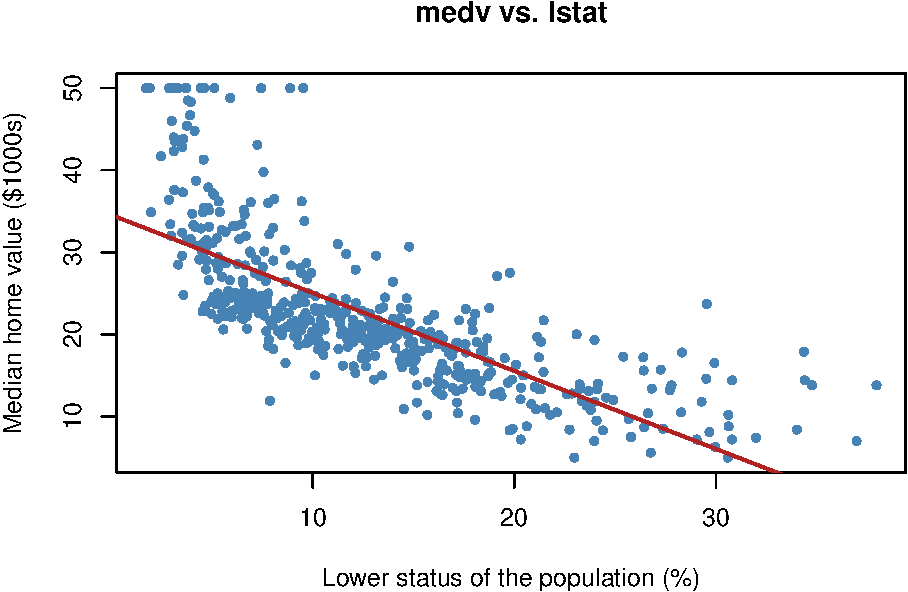
\includegraphics{ch03_lab_files/figure-latex/plot-fit-1} \end{center}

Some extra styling options for \texttt{plot()} and \texttt{abline()}:

\begin{Shaded}
\begin{Highlighting}[]
\FunctionTok{par}\NormalTok{(}\AttributeTok{mfrow =} \FunctionTok{c}\NormalTok{(}\DecValTok{2}\NormalTok{, }\DecValTok{2}\NormalTok{))}
\FunctionTok{plot}\NormalTok{(Boston}\SpecialCharTok{$}\NormalTok{lstat, Boston}\SpecialCharTok{$}\NormalTok{medv, }\AttributeTok{col =} \StringTok{"steelblue"}\NormalTok{, }\AttributeTok{pch =} \DecValTok{20}\NormalTok{)}
\FunctionTok{plot}\NormalTok{(Boston}\SpecialCharTok{$}\NormalTok{lstat, Boston}\SpecialCharTok{$}\NormalTok{medv, }\AttributeTok{pch =} \StringTok{"+"}\NormalTok{)}
\FunctionTok{plot}\NormalTok{(}\DecValTok{1}\SpecialCharTok{:}\DecValTok{20}\NormalTok{, }\DecValTok{1}\SpecialCharTok{:}\DecValTok{20}\NormalTok{, }\AttributeTok{pch =} \DecValTok{1}\SpecialCharTok{:}\DecValTok{20}\NormalTok{, }\AttributeTok{main =} \StringTok{"Point shapes 1{-}20"}\NormalTok{)}
\FunctionTok{plot}\NormalTok{(Boston}\SpecialCharTok{$}\NormalTok{lstat, Boston}\SpecialCharTok{$}\NormalTok{medv, }\AttributeTok{pch =} \DecValTok{20}\NormalTok{, }\AttributeTok{cex =} \FloatTok{0.6}\NormalTok{)}
\end{Highlighting}
\end{Shaded}

\begin{center}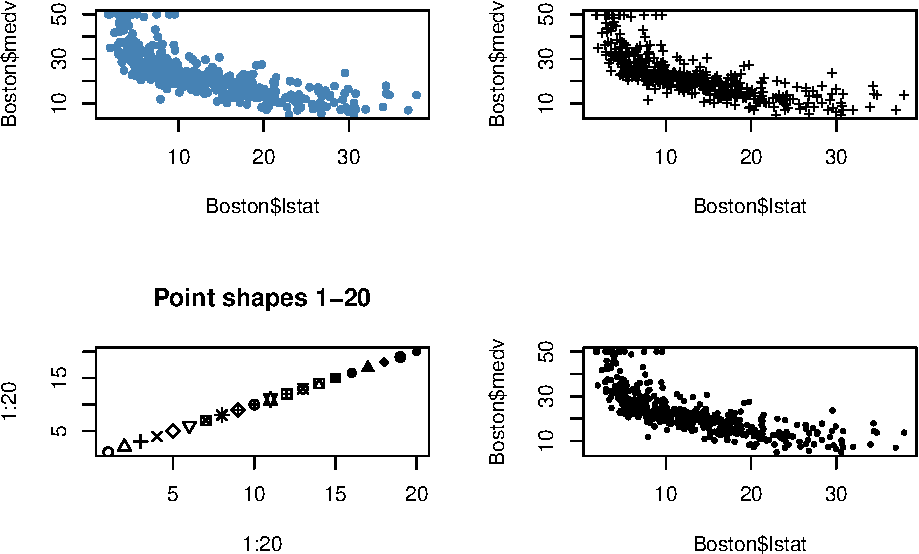
\includegraphics{ch03_lab_files/figure-latex/plot-styles-1} \end{center}

\subsection{Diagnostic plots}\label{diagnostic-plots}

Base R's \texttt{plot()} applied directly to a fitted \texttt{lm} object
produces four standard diagnostic plots: residuals vs.~fitted, a Q-Q
plot, scale-location, and residuals vs.~leverage.

\begin{Shaded}
\begin{Highlighting}[]
\FunctionTok{par}\NormalTok{(}\AttributeTok{mfrow =} \FunctionTok{c}\NormalTok{(}\DecValTok{2}\NormalTok{, }\DecValTok{2}\NormalTok{))}
\FunctionTok{plot}\NormalTok{(lm.fit)}
\end{Highlighting}
\end{Shaded}

\begin{center}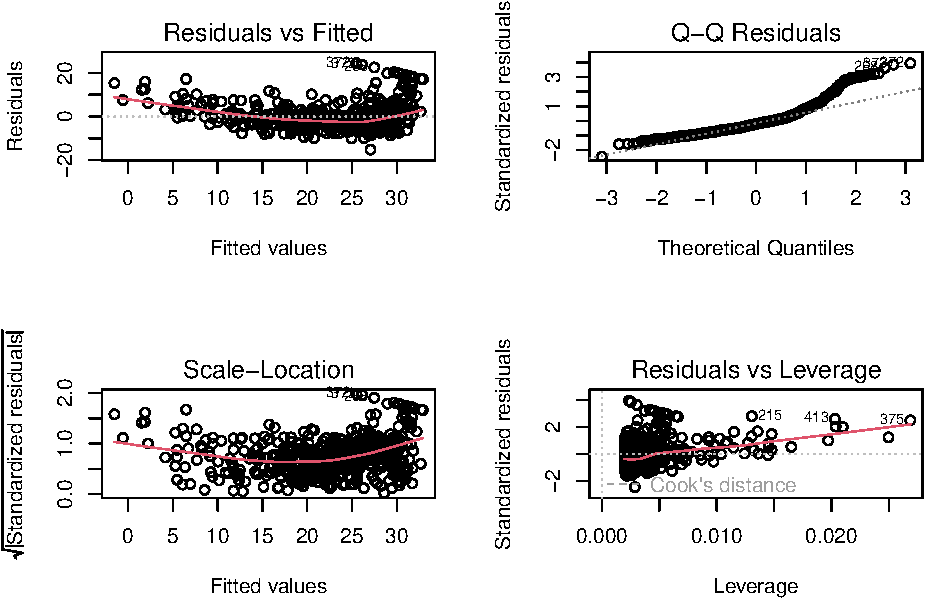
\includegraphics{ch03_lab_files/figure-latex/diagnostics-1} \end{center}

We can also compute residuals and studentized residuals manually, and
inspect leverage statistics:

\begin{Shaded}
\begin{Highlighting}[]
\FunctionTok{par}\NormalTok{(}\AttributeTok{mfrow =} \FunctionTok{c}\NormalTok{(}\DecValTok{1}\NormalTok{, }\DecValTok{1}\NormalTok{))}
\FunctionTok{plot}\NormalTok{(}\FunctionTok{predict}\NormalTok{(lm.fit), }\FunctionTok{residuals}\NormalTok{(lm.fit),}
     \AttributeTok{xlab =} \StringTok{"Fitted values"}\NormalTok{, }\AttributeTok{ylab =} \StringTok{"Residuals"}\NormalTok{)}
\FunctionTok{abline}\NormalTok{(}\AttributeTok{h =} \DecValTok{0}\NormalTok{, }\AttributeTok{lty =} \DecValTok{2}\NormalTok{)}
\end{Highlighting}
\end{Shaded}

\begin{center}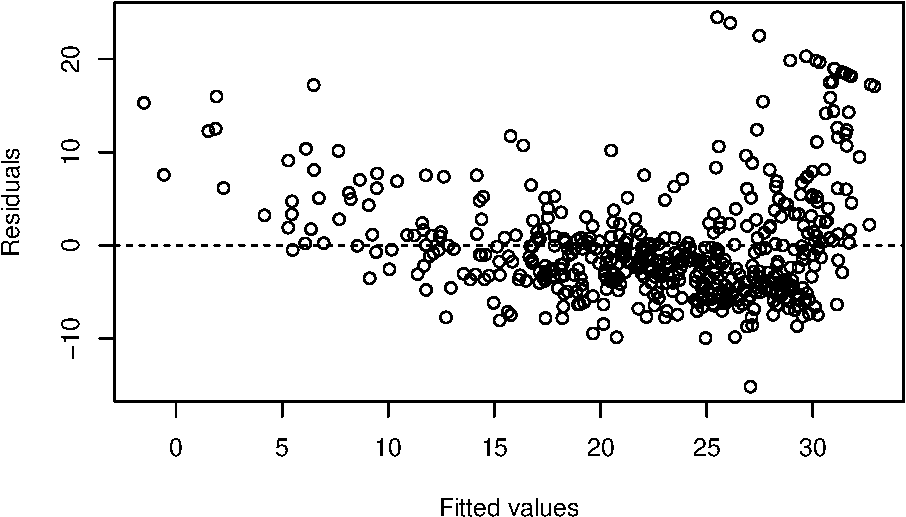
\includegraphics{ch03_lab_files/figure-latex/residuals-leverage-1} \end{center}

\begin{Shaded}
\begin{Highlighting}[]
\FunctionTok{plot}\NormalTok{(}\FunctionTok{predict}\NormalTok{(lm.fit), }\FunctionTok{rstudent}\NormalTok{(lm.fit),}
     \AttributeTok{xlab =} \StringTok{"Fitted values"}\NormalTok{, }\AttributeTok{ylab =} \StringTok{"Studentized residuals"}\NormalTok{)}
\FunctionTok{abline}\NormalTok{(}\AttributeTok{h =} \DecValTok{0}\NormalTok{, }\AttributeTok{lty =} \DecValTok{2}\NormalTok{)}
\end{Highlighting}
\end{Shaded}

\begin{center}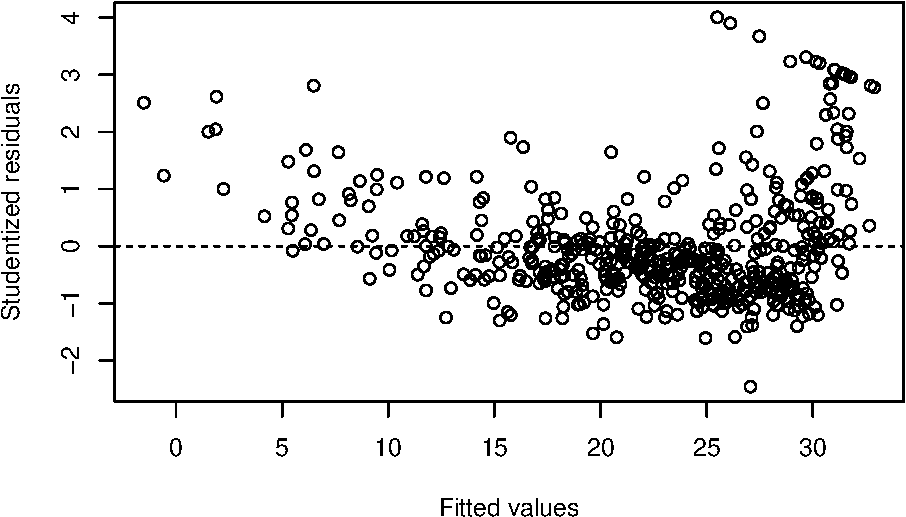
\includegraphics{ch03_lab_files/figure-latex/residuals-leverage-2} \end{center}

\begin{Shaded}
\begin{Highlighting}[]
\CommentTok{\# Leverage statistics {-}{-} which observations have unusually high leverage?}
\FunctionTok{plot}\NormalTok{(}\FunctionTok{hatvalues}\NormalTok{(lm.fit),}
     \AttributeTok{ylab =} \StringTok{"Leverage"}\NormalTok{, }\AttributeTok{main =} \StringTok{"Leverage by observation"}\NormalTok{)}
\end{Highlighting}
\end{Shaded}

\begin{center}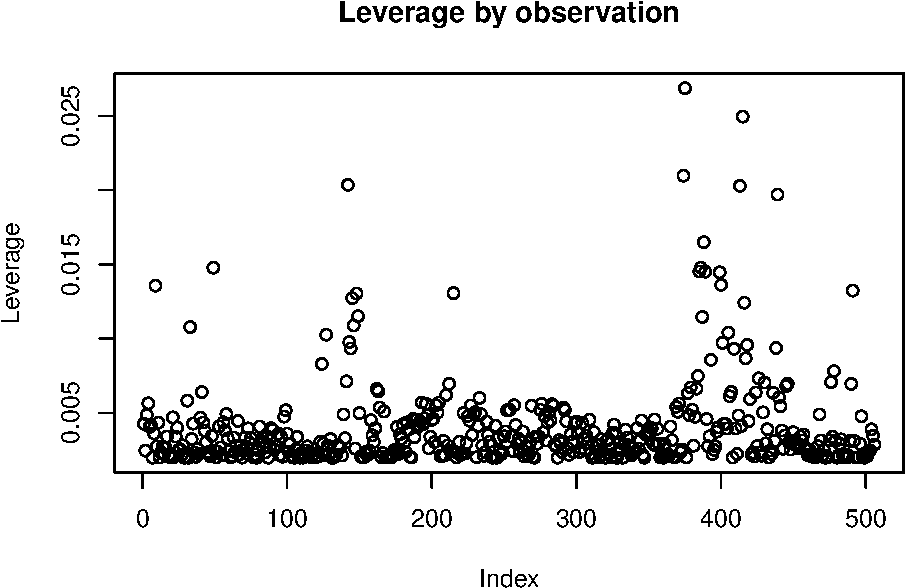
\includegraphics{ch03_lab_files/figure-latex/residuals-leverage-3} \end{center}

\begin{Shaded}
\begin{Highlighting}[]
\FunctionTok{which.max}\NormalTok{(}\FunctionTok{hatvalues}\NormalTok{(lm.fit))}
\end{Highlighting}
\end{Shaded}

\begin{verbatim}
## 375 
## 375
\end{verbatim}

\section{Multiple Linear Regression}\label{multiple-linear-regression}

A single predictor rarely tells the whole story --- \texttt{medv}
plausibly depends on more than just \texttt{lstat}. Multiple linear
regression extends the same least-squares idea to \(p\) predictors:

\[
\text{medv} = \beta_0 + \beta_1 X_1 + \beta_2 X_2 + \cdots + \beta_p X_p + \epsilon
\]

Each \(\hat\beta_j\) is now interpreted as the effect of a one-unit
increase in \(X_j\) \emph{holding all other predictors fixed} --- a
different reading than in simple regression, where \(\hat\beta_1\)
captured \(X_1\)'s effect with nothing else in the model to hold
constant.

Now we extend the model to include more than one predictor.

\begin{Shaded}
\begin{Highlighting}[]
\NormalTok{lm.fit2 }\OtherTok{\textless{}{-}} \FunctionTok{lm}\NormalTok{(medv }\SpecialCharTok{\textasciitilde{}}\NormalTok{ lstat }\SpecialCharTok{+}\NormalTok{ age, }\AttributeTok{data =}\NormalTok{ Boston)}
\FunctionTok{summary}\NormalTok{(lm.fit2)}
\end{Highlighting}
\end{Shaded}

\begin{verbatim}
## 
## Call:
## lm(formula = medv ~ lstat + age, data = Boston)
## 
## Residuals:
##     Min      1Q  Median      3Q     Max 
## -15.981  -3.978  -1.283   1.968  23.158 
## 
## Coefficients:
##             Estimate Std. Error t value Pr(>|t|)    
## (Intercept) 33.22276    0.73085  45.458  < 2e-16 ***
## lstat       -1.03207    0.04819 -21.416  < 2e-16 ***
## age          0.03454    0.01223   2.826  0.00491 ** 
## ---
## Signif. codes:  0 '***' 0.001 '**' 0.01 '*' 0.05 '.' 0.1 ' ' 1
## 
## Residual standard error: 6.173 on 503 degrees of freedom
## Multiple R-squared:  0.5513, Adjusted R-squared:  0.5495 
## F-statistic:   309 on 2 and 503 DF,  p-value: < 2.2e-16
\end{verbatim}

\subsection{Using all predictors}\label{using-all-predictors}

Rather than typing every variable name, we can regress \texttt{medv} on
all other variables in the data frame using \texttt{.}:

\begin{Shaded}
\begin{Highlighting}[]
\NormalTok{lm.fit.all }\OtherTok{\textless{}{-}} \FunctionTok{lm}\NormalTok{(medv }\SpecialCharTok{\textasciitilde{}}\NormalTok{ ., }\AttributeTok{data =}\NormalTok{ Boston)}
\FunctionTok{summary}\NormalTok{(lm.fit.all)}
\end{Highlighting}
\end{Shaded}

\begin{verbatim}
## 
## Call:
## lm(formula = medv ~ ., data = Boston)
## 
## Residuals:
##      Min       1Q   Median       3Q      Max 
## -15.1304  -2.7673  -0.5814   1.9414  26.2526 
## 
## Coefficients:
##               Estimate Std. Error t value Pr(>|t|)    
## (Intercept)  41.617270   4.936039   8.431 3.79e-16 ***
## crim         -0.121389   0.033000  -3.678 0.000261 ***
## zn            0.046963   0.013879   3.384 0.000772 ***
## indus         0.013468   0.062145   0.217 0.828520    
## chas          2.839993   0.870007   3.264 0.001173 ** 
## nox         -18.758022   3.851355  -4.870 1.50e-06 ***
## rm            3.658119   0.420246   8.705  < 2e-16 ***
## age           0.003611   0.013329   0.271 0.786595    
## dis          -1.490754   0.201623  -7.394 6.17e-13 ***
## rad           0.289405   0.066908   4.325 1.84e-05 ***
## tax          -0.012682   0.003801  -3.337 0.000912 ***
## ptratio      -0.937533   0.132206  -7.091 4.63e-12 ***
## lstat        -0.552019   0.050659 -10.897  < 2e-16 ***
## ---
## Signif. codes:  0 '***' 0.001 '**' 0.01 '*' 0.05 '.' 0.1 ' ' 1
## 
## Residual standard error: 4.798 on 493 degrees of freedom
## Multiple R-squared:  0.7343, Adjusted R-squared:  0.7278 
## F-statistic: 113.5 on 12 and 493 DF,  p-value: < 2.2e-16
\end{verbatim}

We can access individual pieces of the summary object, such as \(R^2\)
and the residual standard error:

\begin{Shaded}
\begin{Highlighting}[]
\FunctionTok{summary}\NormalTok{(lm.fit.all)}\SpecialCharTok{$}\NormalTok{r.squared}
\end{Highlighting}
\end{Shaded}

\begin{verbatim}
## [1] 0.734307
\end{verbatim}

\begin{Shaded}
\begin{Highlighting}[]
\FunctionTok{summary}\NormalTok{(lm.fit.all)}\SpecialCharTok{$}\NormalTok{sigma}
\end{Highlighting}
\end{Shaded}

\begin{verbatim}
## [1] 4.798034
\end{verbatim}

\subsection{Checking for
multicollinearity}\label{checking-for-multicollinearity}

Variance inflation factors (VIFs) help flag predictors that are highly
correlated with other predictors, which can inflate coefficient standard
errors. For predictor \(X_j\), the VIF is defined using \(R^2_{X_j}\)
--- the \(R^2\) from regressing \(X_j\) on \emph{all the other
predictors}:

\[
\text{VIF}(\hat\beta_j) = \frac{1}{1 - R^2_{X_j}}
\]

If \(X_j\) is well explained by the other predictors (\(R^2_{X_j}\)
close to 1), the denominator shrinks toward 0 and the VIF blows up --- a
sign that \(X_j\)'s own coefficient estimate is unstable because the
data can't cleanly separate its effect from the other predictors it's
correlated with. A VIF of 1 means no collinearity at all; VIFs above
roughly 5--10 are typically treated as cause for concern.

\begin{Shaded}
\begin{Highlighting}[]
\FunctionTok{vif}\NormalTok{(lm.fit.all)}
\end{Highlighting}
\end{Shaded}

\begin{verbatim}
##     crim       zn    indus     chas      nox       rm      age      dis 
## 1.767486 2.298459 3.987181 1.071168 4.369093 1.912532 3.088232 3.954037 
##      rad      tax  ptratio    lstat 
## 7.445301 9.002158 1.797060 2.870777
\end{verbatim}

\subsection{Fitting with one predictor
excluded}\label{fitting-with-one-predictor-excluded}

Suppose we want to fit the model using all predictors except one (say,
\texttt{age}, which had a very high p-value above). We can do this two
ways:

\begin{Shaded}
\begin{Highlighting}[]
\NormalTok{lm.fit.no.age }\OtherTok{\textless{}{-}} \FunctionTok{lm}\NormalTok{(medv }\SpecialCharTok{\textasciitilde{}}\NormalTok{ . }\SpecialCharTok{{-}}\NormalTok{ age, }\AttributeTok{data =}\NormalTok{ Boston)}
\FunctionTok{summary}\NormalTok{(lm.fit.no.age)}
\end{Highlighting}
\end{Shaded}

\begin{verbatim}
## 
## Call:
## lm(formula = medv ~ . - age, data = Boston)
## 
## Residuals:
##      Min       1Q   Median       3Q      Max 
## -15.1851  -2.7330  -0.6116   1.8555  26.3838 
## 
## Coefficients:
##               Estimate Std. Error t value Pr(>|t|)    
## (Intercept)  41.525128   4.919684   8.441 3.52e-16 ***
## crim         -0.121426   0.032969  -3.683 0.000256 ***
## zn            0.046512   0.013766   3.379 0.000785 ***
## indus         0.013451   0.062086   0.217 0.828577    
## chas          2.852773   0.867912   3.287 0.001085 ** 
## nox         -18.485070   3.713714  -4.978 8.91e-07 ***
## rm            3.681070   0.411230   8.951  < 2e-16 ***
## dis          -1.506777   0.192570  -7.825 3.12e-14 ***
## rad           0.287940   0.066627   4.322 1.87e-05 ***
## tax          -0.012653   0.003796  -3.333 0.000923 ***
## ptratio      -0.934649   0.131653  -7.099 4.39e-12 ***
## lstat        -0.547409   0.047669 -11.483  < 2e-16 ***
## ---
## Signif. codes:  0 '***' 0.001 '**' 0.01 '*' 0.05 '.' 0.1 ' ' 1
## 
## Residual standard error: 4.794 on 494 degrees of freedom
## Multiple R-squared:  0.7343, Adjusted R-squared:  0.7284 
## F-statistic: 124.1 on 11 and 494 DF,  p-value: < 2.2e-16
\end{verbatim}

\begin{Shaded}
\begin{Highlighting}[]
\CommentTok{\# Equivalently, using update() on an existing fit:}
\NormalTok{lm.fit.updated }\OtherTok{\textless{}{-}} \FunctionTok{update}\NormalTok{(lm.fit.all, }\SpecialCharTok{\textasciitilde{}}\NormalTok{ . }\SpecialCharTok{{-}}\NormalTok{ age)}
\FunctionTok{summary}\NormalTok{(lm.fit.updated)}
\end{Highlighting}
\end{Shaded}

\begin{verbatim}
## 
## Call:
## lm(formula = medv ~ crim + zn + indus + chas + nox + rm + dis + 
##     rad + tax + ptratio + lstat, data = Boston)
## 
## Residuals:
##      Min       1Q   Median       3Q      Max 
## -15.1851  -2.7330  -0.6116   1.8555  26.3838 
## 
## Coefficients:
##               Estimate Std. Error t value Pr(>|t|)    
## (Intercept)  41.525128   4.919684   8.441 3.52e-16 ***
## crim         -0.121426   0.032969  -3.683 0.000256 ***
## zn            0.046512   0.013766   3.379 0.000785 ***
## indus         0.013451   0.062086   0.217 0.828577    
## chas          2.852773   0.867912   3.287 0.001085 ** 
## nox         -18.485070   3.713714  -4.978 8.91e-07 ***
## rm            3.681070   0.411230   8.951  < 2e-16 ***
## dis          -1.506777   0.192570  -7.825 3.12e-14 ***
## rad           0.287940   0.066627   4.322 1.87e-05 ***
## tax          -0.012653   0.003796  -3.333 0.000923 ***
## ptratio      -0.934649   0.131653  -7.099 4.39e-12 ***
## lstat        -0.547409   0.047669 -11.483  < 2e-16 ***
## ---
## Signif. codes:  0 '***' 0.001 '**' 0.01 '*' 0.05 '.' 0.1 ' ' 1
## 
## Residual standard error: 4.794 on 494 degrees of freedom
## Multiple R-squared:  0.7343, Adjusted R-squared:  0.7284 
## F-statistic: 124.1 on 11 and 494 DF,  p-value: < 2.2e-16
\end{verbatim}

\section{Interaction Terms}\label{interaction-terms}

Additive multiple regression assumes each predictor's effect is
independent of the others --- the effect of \texttt{lstat} on
\texttt{medv} is the same whichever value \texttt{age} happens to take.
An interaction term relaxes that assumption:

\[
\text{medv} = \beta_0 + \beta_1 \cdot \text{lstat} + \beta_2 \cdot \text{age} + \beta_3 \cdot (\text{lstat} \times \text{age}) + \epsilon
\]

Rearranging the \texttt{lstat} terms makes the point concrete ---
\texttt{lstat}'s effective slope now depends on the value of
\texttt{age}:

\[
\text{medv} = \beta_0 + (\beta_1 + \beta_3 \cdot \text{age}) \cdot \text{lstat} + \beta_2 \cdot \text{age} + \epsilon
\]

\texttt{lstat:age} includes only the interaction term (\(\beta_3\)),
while \texttt{lstat*age} is shorthand for
\texttt{lstat\ +\ age\ +\ lstat:age} -- i.e., it includes both main
effects and the interaction, matching the full formula above.

\begin{Shaded}
\begin{Highlighting}[]
\FunctionTok{summary}\NormalTok{(}\FunctionTok{lm}\NormalTok{(medv }\SpecialCharTok{\textasciitilde{}}\NormalTok{ lstat }\SpecialCharTok{*}\NormalTok{ age, }\AttributeTok{data =}\NormalTok{ Boston))}
\end{Highlighting}
\end{Shaded}

\begin{verbatim}
## 
## Call:
## lm(formula = medv ~ lstat * age, data = Boston)
## 
## Residuals:
##     Min      1Q  Median      3Q     Max 
## -15.806  -4.045  -1.333   2.085  27.552 
## 
## Coefficients:
##               Estimate Std. Error t value Pr(>|t|)    
## (Intercept) 36.0885359  1.4698355  24.553  < 2e-16 ***
## lstat       -1.3921168  0.1674555  -8.313 8.78e-16 ***
## age         -0.0007209  0.0198792  -0.036   0.9711    
## lstat:age    0.0041560  0.0018518   2.244   0.0252 *  
## ---
## Signif. codes:  0 '***' 0.001 '**' 0.01 '*' 0.05 '.' 0.1 ' ' 1
## 
## Residual standard error: 6.149 on 502 degrees of freedom
## Multiple R-squared:  0.5557, Adjusted R-squared:  0.5531 
## F-statistic: 209.3 on 3 and 502 DF,  p-value: < 2.2e-16
\end{verbatim}

\section{Non-linear Transformations of
Predictors}\label{non-linear-transformations-of-predictors}

The \texttt{lm()} function can accommodate non-linear transformations of
predictors directly in the formula, using \texttt{I()} to protect
arithmetic operators like \texttt{\^{}} from being interpreted as
formula syntax.

\[
\text{medv} = \beta_0 + \beta_1 \cdot \text{lstat} + \beta_2 \cdot \text{lstat}^2 + \epsilon
\]

This is still a \emph{linear} model in the statistical sense --- linear
in the parameters \(\beta_0, \beta_1, \beta_2\) --- even though the
fitted curve itself is not a straight line. That's exactly why
\texttt{lm()} can fit it directly.

\begin{Shaded}
\begin{Highlighting}[]
\NormalTok{lm.fit.sq }\OtherTok{\textless{}{-}} \FunctionTok{lm}\NormalTok{(medv }\SpecialCharTok{\textasciitilde{}}\NormalTok{ lstat }\SpecialCharTok{+} \FunctionTok{I}\NormalTok{(lstat}\SpecialCharTok{\^{}}\DecValTok{2}\NormalTok{), }\AttributeTok{data =}\NormalTok{ Boston)}
\FunctionTok{summary}\NormalTok{(lm.fit.sq)}
\end{Highlighting}
\end{Shaded}

\begin{verbatim}
## 
## Call:
## lm(formula = medv ~ lstat + I(lstat^2), data = Boston)
## 
## Residuals:
##      Min       1Q   Median       3Q      Max 
## -15.2834  -3.8313  -0.5295   2.3095  25.4148 
## 
## Coefficients:
##              Estimate Std. Error t value Pr(>|t|)    
## (Intercept) 42.862007   0.872084   49.15   <2e-16 ***
## lstat       -2.332821   0.123803  -18.84   <2e-16 ***
## I(lstat^2)   0.043547   0.003745   11.63   <2e-16 ***
## ---
## Signif. codes:  0 '***' 0.001 '**' 0.01 '*' 0.05 '.' 0.1 ' ' 1
## 
## Residual standard error: 5.524 on 503 degrees of freedom
## Multiple R-squared:  0.6407, Adjusted R-squared:  0.6393 
## F-statistic: 448.5 on 2 and 503 DF,  p-value: < 2.2e-16
\end{verbatim}

We can use \texttt{anova()} to formally compare the linear-only model to
the model that also includes the quadratic term:

\begin{Shaded}
\begin{Highlighting}[]
\NormalTok{lm.fit.linear }\OtherTok{\textless{}{-}} \FunctionTok{lm}\NormalTok{(medv }\SpecialCharTok{\textasciitilde{}}\NormalTok{ lstat, }\AttributeTok{data =}\NormalTok{ Boston)}
\FunctionTok{anova}\NormalTok{(lm.fit.linear, lm.fit.sq)}
\end{Highlighting}
\end{Shaded}

\begin{verbatim}
## Analysis of Variance Table
## 
## Model 1: medv ~ lstat
## Model 2: medv ~ lstat + I(lstat^2)
##   Res.Df   RSS Df Sum of Sq     F    Pr(>F)    
## 1    504 19472                                 
## 2    503 15347  1    4125.1 135.2 < 2.2e-16 ***
## ---
## Signif. codes:  0 '***' 0.001 '**' 0.01 '*' 0.05 '.' 0.1 ' ' 1
\end{verbatim}

\begin{Shaded}
\begin{Highlighting}[]
\FunctionTok{par}\NormalTok{(}\AttributeTok{mfrow =} \FunctionTok{c}\NormalTok{(}\DecValTok{2}\NormalTok{, }\DecValTok{2}\NormalTok{))}
\FunctionTok{plot}\NormalTok{(lm.fit.sq)}
\end{Highlighting}
\end{Shaded}

\begin{center}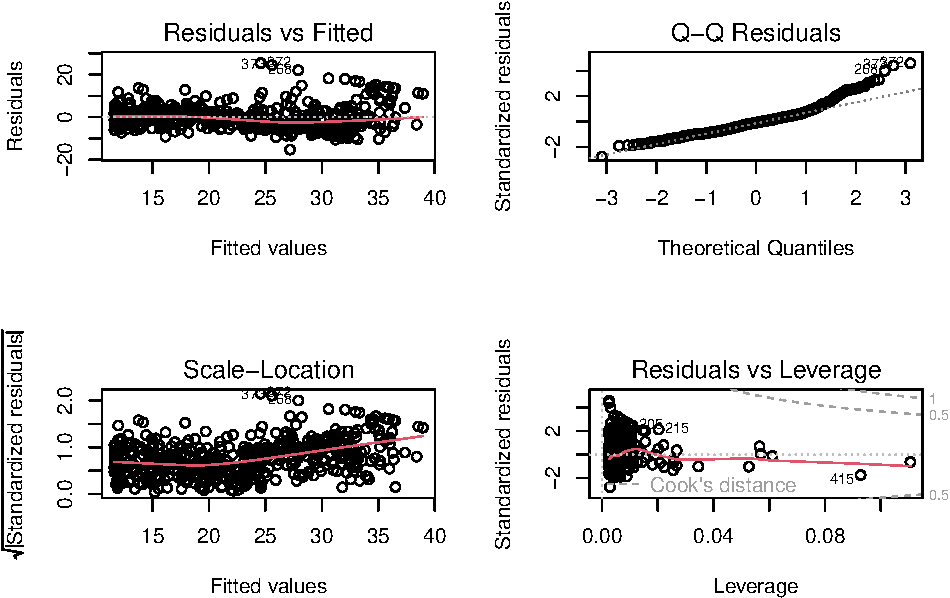
\includegraphics{ch03_lab_files/figure-latex/poly-diagnostics-1} \end{center}

For a higher-order polynomial fit, the \texttt{poly()} function is more
convenient than writing out each \texttt{I(lstat\^{}k)} term by hand:

\begin{Shaded}
\begin{Highlighting}[]
\NormalTok{lm.fit.poly5 }\OtherTok{\textless{}{-}} \FunctionTok{lm}\NormalTok{(medv }\SpecialCharTok{\textasciitilde{}} \FunctionTok{poly}\NormalTok{(lstat, }\DecValTok{5}\NormalTok{), }\AttributeTok{data =}\NormalTok{ Boston)}
\FunctionTok{summary}\NormalTok{(lm.fit.poly5)}
\end{Highlighting}
\end{Shaded}

\begin{verbatim}
## 
## Call:
## lm(formula = medv ~ poly(lstat, 5), data = Boston)
## 
## Residuals:
##      Min       1Q   Median       3Q      Max 
## -13.5433  -3.1039  -0.7052   2.0844  27.1153 
## 
## Coefficients:
##                  Estimate Std. Error t value Pr(>|t|)    
## (Intercept)       22.5328     0.2318  97.197  < 2e-16 ***
## poly(lstat, 5)1 -152.4595     5.2148 -29.236  < 2e-16 ***
## poly(lstat, 5)2   64.2272     5.2148  12.316  < 2e-16 ***
## poly(lstat, 5)3  -27.0511     5.2148  -5.187 3.10e-07 ***
## poly(lstat, 5)4   25.4517     5.2148   4.881 1.42e-06 ***
## poly(lstat, 5)5  -19.2524     5.2148  -3.692 0.000247 ***
## ---
## Signif. codes:  0 '***' 0.001 '**' 0.01 '*' 0.05 '.' 0.1 ' ' 1
## 
## Residual standard error: 5.215 on 500 degrees of freedom
## Multiple R-squared:  0.6817, Adjusted R-squared:  0.6785 
## F-statistic: 214.2 on 5 and 500 DF,  p-value: < 2.2e-16
\end{verbatim}

We can also try a log transformation of a predictor:

\begin{Shaded}
\begin{Highlighting}[]
\FunctionTok{summary}\NormalTok{(}\FunctionTok{lm}\NormalTok{(medv }\SpecialCharTok{\textasciitilde{}} \FunctionTok{log}\NormalTok{(rm), }\AttributeTok{data =}\NormalTok{ Boston))}
\end{Highlighting}
\end{Shaded}

\begin{verbatim}
## 
## Call:
## lm(formula = medv ~ log(rm), data = Boston)
## 
## Residuals:
##     Min      1Q  Median      3Q     Max 
## -19.487  -2.875  -0.104   2.837  39.816 
## 
## Coefficients:
##             Estimate Std. Error t value Pr(>|t|)    
## (Intercept)  -76.488      5.028  -15.21   <2e-16 ***
## log(rm)       54.055      2.739   19.73   <2e-16 ***
## ---
## Signif. codes:  0 '***' 0.001 '**' 0.01 '*' 0.05 '.' 0.1 ' ' 1
## 
## Residual standard error: 6.915 on 504 degrees of freedom
## Multiple R-squared:  0.4358, Adjusted R-squared:  0.4347 
## F-statistic: 389.3 on 1 and 504 DF,  p-value: < 2.2e-16
\end{verbatim}

\section{Qualitative Predictors}\label{qualitative-predictors}

We switch to the \texttt{Carseats} data set, which includes a mix of
quantitative and qualitative (categorical) predictors, to demonstrate
how \texttt{lm()} handles factor variables.

\begin{Shaded}
\begin{Highlighting}[]
\NormalTok{Carseats }\OtherTok{\textless{}{-}}\NormalTok{ ISLR2}\SpecialCharTok{::}\NormalTok{Carseats}
\FunctionTok{str}\NormalTok{(Carseats)}
\end{Highlighting}
\end{Shaded}

\begin{verbatim}
## 'data.frame':    400 obs. of  11 variables:
##  $ Sales      : num  9.5 11.22 10.06 7.4 4.15 ...
##  $ CompPrice  : num  138 111 113 117 141 124 115 136 132 132 ...
##  $ Income     : num  73 48 35 100 64 113 105 81 110 113 ...
##  $ Advertising: num  11 16 10 4 3 13 0 15 0 0 ...
##  $ Population : num  276 260 269 466 340 501 45 425 108 131 ...
##  $ Price      : num  120 83 80 97 128 72 108 120 124 124 ...
##  $ ShelveLoc  : Factor w/ 3 levels "Bad","Good","Medium": 1 2 3 3 1 1 3 2 3 3 ...
##  $ Age        : num  42 65 59 55 38 78 71 67 76 76 ...
##  $ Education  : num  17 10 12 14 13 16 15 10 10 17 ...
##  $ Urban      : Factor w/ 2 levels "No","Yes": 2 2 2 2 2 1 2 2 1 1 ...
##  $ US         : Factor w/ 2 levels "No","Yes": 2 2 2 2 1 2 1 2 1 2 ...
\end{verbatim}

\subsection{Fitting a model with interactions and a factor
variable}\label{fitting-a-model-with-interactions-and-a-factor-variable}

\begin{Shaded}
\begin{Highlighting}[]
\NormalTok{lm.fit.carseats }\OtherTok{\textless{}{-}} \FunctionTok{lm}\NormalTok{(Sales }\SpecialCharTok{\textasciitilde{}}\NormalTok{ . }\SpecialCharTok{+}\NormalTok{ Income}\SpecialCharTok{:}\NormalTok{Advertising }\SpecialCharTok{+}\NormalTok{ Price}\SpecialCharTok{:}\NormalTok{Age,}
                       \AttributeTok{data =}\NormalTok{ Carseats)}
\FunctionTok{summary}\NormalTok{(lm.fit.carseats)}
\end{Highlighting}
\end{Shaded}

\begin{verbatim}
## 
## Call:
## lm(formula = Sales ~ . + Income:Advertising + Price:Age, data = Carseats)
## 
## Residuals:
##     Min      1Q  Median      3Q     Max 
## -2.9208 -0.7503  0.0177  0.6754  3.3413 
## 
## Coefficients:
##                      Estimate Std. Error t value Pr(>|t|)    
## (Intercept)         6.5755654  1.0087470   6.519 2.22e-10 ***
## CompPrice           0.0929371  0.0041183  22.567  < 2e-16 ***
## Income              0.0108940  0.0026044   4.183 3.57e-05 ***
## Advertising         0.0702462  0.0226091   3.107 0.002030 ** 
## Population          0.0001592  0.0003679   0.433 0.665330    
## Price              -0.1008064  0.0074399 -13.549  < 2e-16 ***
## ShelveLocGood       4.8486762  0.1528378  31.724  < 2e-16 ***
## ShelveLocMedium     1.9532620  0.1257682  15.531  < 2e-16 ***
## Age                -0.0579466  0.0159506  -3.633 0.000318 ***
## Education          -0.0208525  0.0196131  -1.063 0.288361    
## UrbanYes            0.1401597  0.1124019   1.247 0.213171    
## USYes              -0.1575571  0.1489234  -1.058 0.290729    
## Income:Advertising  0.0007510  0.0002784   2.698 0.007290 ** 
## Price:Age           0.0001068  0.0001333   0.801 0.423812    
## ---
## Signif. codes:  0 '***' 0.001 '**' 0.01 '*' 0.05 '.' 0.1 ' ' 1
## 
## Residual standard error: 1.011 on 386 degrees of freedom
## Multiple R-squared:  0.8761, Adjusted R-squared:  0.8719 
## F-statistic:   210 on 13 and 386 DF,  p-value: < 2.2e-16
\end{verbatim}

R automatically creates dummy variables for qualitative predictors such
as \texttt{ShelveLoc} (a three-level factor: \texttt{Bad},
\texttt{Medium}, \texttt{Good}). With \(k=3\) levels, R creates
\(k-1=2\) dummy variables and folds their coefficients into the same
linear model:

\[
\text{Sales} = \beta_0 + \beta_1 \cdot X_{\text{Good}} + \beta_2 \cdot X_{\text{Medium}} + \cdots + \epsilon,
\qquad X_{\text{Good}} =
\begin{cases} 1 & \text{if ShelveLoc = Good} \\ 0 & \text{otherwise} \end{cases}
\]

(and similarly for \(X_{\text{Medium}}\)). The omitted level,
\texttt{Bad}, becomes the baseline: when both dummies are 0, the model's
intercept \(\beta_0\) represents a \texttt{Bad} shelf location, so
\(\beta_1\) and \(\beta_2\) are read as the shift in expected
\texttt{Sales} \emph{relative to} \texttt{Bad}, not as standalone
effects. We can check how these dummy variables were coded using
\texttt{contrasts()}:

\begin{Shaded}
\begin{Highlighting}[]
\FunctionTok{contrasts}\NormalTok{(Carseats}\SpecialCharTok{$}\NormalTok{ShelveLoc)}
\end{Highlighting}
\end{Shaded}

\begin{verbatim}
##        Good Medium
## Bad       0      0
## Good      1      0
## Medium    0      1
\end{verbatim}

The coefficients on \texttt{ShelveLocGood} and \texttt{ShelveLocMedium}
represent the expected change in sales relative to the baseline level
(\texttt{Bad} shelf location), holding all other predictors fixed.

\section{Writing a Small Function}\label{writing-a-small-function}

Finally, a short example of writing our own function -- here, one that
loads several packages at once, which can be handy at the start of a
script or report like this one.

\begin{Shaded}
\begin{Highlighting}[]
\NormalTok{LoadLibraries }\OtherTok{\textless{}{-}} \ControlFlowTok{function}\NormalTok{() \{}
  \FunctionTok{library}\NormalTok{(ISLR2)}
  \FunctionTok{library}\NormalTok{(MASS)}
  \FunctionTok{library}\NormalTok{(car)}
  \FunctionTok{print}\NormalTok{(}\StringTok{"The libraries have been loaded."}\NormalTok{)}
\NormalTok{\}}

\FunctionTok{LoadLibraries}\NormalTok{()}
\end{Highlighting}
\end{Shaded}

\begin{verbatim}
## [1] "The libraries have been loaded."
\end{verbatim}

\section{Summary}\label{summary}

In this lab we:

\begin{enumerate}
\def\labelenumi{\arabic{enumi}.}
\tightlist
\item
  Fit and interpreted simple and multiple linear regression models.
\item
  Computed confidence and prediction intervals for predicted responses.
\item
  Produced and interpreted standard regression diagnostic plots.
\item
  Checked for multicollinearity using variance inflation factors.
\item
  Added interaction terms and non-linear (polynomial, log)
  transformations.
\item
  Incorporated qualitative predictors and inspected their dummy-variable
  coding.
\end{enumerate}

These tools form the foundation for the more flexible modeling
approaches covered in later chapters.

\end{document}
